\section{Calculation von Neumann}
Since our motivations are about physics and realistic 
future implementations, we try to connect our abstract calculations to 
example states already produced in experiments. Firstly we calculate the vonNeumann entropy of a so-called maximally entangled state. As an experimental example we use the state:
\begin{equation}
|\psi\rangle=\frac{|H\rangle|x+\rangle-i|V\rangle|x-\rangle}{\sqrt{2}}
\label{psivon}
\end{equation}
from \cite{PhysRevLett.110.167401}. Here $\ket{H}$ and $\ket{V}$ denote the
horizontal and vertical polarization of light while $\ket{x\pm}$ are ground and excited states a singly charged superconductor quantum dot. The convention is usually to denote as $\ket{0}$ the horizontal polarization and down(minus) spin of the quantum dot. Hence the state takes the form:
\begin{equation}
|\psi\rangle=\frac{|01\rangle-i|10\rangle}{\sqrt{2}}=\frac{1}{\sqrt{2}}\left(
\begin{array}{c}
 0 \\
 1\\
 -i\\
 0 \\
\end{array}
\right)
\end{equation}
Hence the density matrix would be:
\begin{align}
\rho &= \ket{\psi} \bra{\psi} \nonumber \\[0.5em]
&=\big{(}|01\rangle-i|10\rangle\big{)}\big{(}\langle01|+i\langle10|\big{)}\\[0.5em]
&=\frac{1}{2}\left(
\begin{array}{cccc}
 0 & 0 & 0 & 0 \\
 0 & 1 & i & 0 \\
 0 & -i & 1 & 0 \\
 0 & 0 & 0 & 0 \\
\end{array}
\right)\nonumber
\end{align}
Now, we write the matrix $\rho$ using its modal matrix and the corresponding diagonal matrix. 
First we calculate the eigenvectors and eigenvalues  of $\rho$.
\begin{equation}
\lambda_1=1,\:  \lambda_2=0,\:  \lambda_3=0,\:  \lambda_4=0, 
\end{equation}
\begin{equation}
v_1=\{0,i,1,0\},\:  v_2=\{0,0,0,1\},\:  v_3= \{0,-i,1,0\},\:  v_4= \{1,0,0,0\}
\end{equation}
Now we readily see that the modal matrix is:
\begin{equation}
M=
\left( \begin{array}{cccc}
 0 & 0 & 0 & 1 \\
 i & 0 & -i & 0 \\
 1 & 0 & 1 & 0 \\
 0 & 1 & 0 & 0 \\
\end{array}
\right)
\end{equation}
which gives us $det(M)=2i$ and : 
\begin{equation}
M^{-1}=\frac{1}{2}
\left( \begin{array}{cccc}
 0 & -i & 1 & 0 \\
 0 & 0 & 0 & 1 \\
 0 & i & 1 & 0 \\
 1 & 0 & 0 & 0 \\
\end{array}
\right).
\end{equation}
So we have decomposed $\rho$ as:
\begin{equation}
\rho=MDM^{-1}
\end{equation}
in which:
\begin{equation}
D=diag(1,0,0,0).
\label{diag}
\end{equation}
Now, using the THEOREM we can seemingly just take the logarithm of the elements of $D$ and finish with the calculation easily. However, looking a little bit closer we run into a problem. In the function $\rho ln \rho$ that gives us the vonNeumman entropy taking $0ln0$ when calculating for each eigenvalue, looks nonsensical at first sight. This is why we basically defined the vonNeumman entropy as in DEFINITION. Taking this into account it is evidently true that for $F(A)=AlnA$:
\begin{align}
S(\rho) &= -\operatorname{Tr}(F(\rho)) \nonumber \\[0.5em]
&= -\operatorname{Tr}(F(MDM^{-1})) \nonumber \\[0.5em]
&=-\operatorname{Tr}\Bigg[
M
\left( \begin{array}{cccc}
 F(1) & 0 & 0 & 0 \\
 0 & F(0) & 0 & 0 \\
 0 & 0 & F(0) & 0 \\
 0 & 0 & 0 & F(0) \\
\end{array}
\right)
M^{-1}
\Bigg]
\nonumber\\[0.5em]
&=0
\end{align}  
The result is of course expected since the vonNeumman entropy is zero if and only if $\rho$ is a pure state.
\section{Conditional entropy calculation}
Now for the Conditional Entropy calculation we will take a different state created experimentally at \cite{gomez2019experimental}. It is a general form of entangled photons looking like:
\begin{equation}
|\psi(\theta)\rangle=\cos (\theta)|00\rangle+\sin (\theta)|11\rangle
\label{condentpsi}
\end{equation}
with $0< \theta< \pi /2$ to ensure entanglement and avoid ill-defined calculations with infinities.
Now we have to calculate both the von Neumann entropy of the whole state, and the von Neumann entropy for the partially traced sub-state that we choose as the conditional. All these, according to the definition \ref{condent}.
From \ref{condentpsi} we deduce its density matrix:
\begin{equation}
\sigma^{AB}=\left(
\begin{array}{cccc}
 cos ^2 \theta & 0 & 0 & cos \theta sin \theta \\
 0 & 0 & 0 & 0 \\
 0 & 0 & 0 & 0 \\
 cos \theta sin \theta & 0 & 0 & sin ^2 \theta  \\
\end{array}
\right)
\end{equation}
We find the eigenvalues and eigenvectors of $\sigma$:

\begin{equation}
\lambda_1=1,\:  \lambda_2=0,\:  \lambda_3=0,\:  \lambda_4=0, 
\end{equation}
\begin{equation}
v_1=\{cot \theta ,0,0,1\},\:  v_2=\{-tan\theta,0,0,1\},\:  v_3= \{0,0,1,0\},\:  v_4= \{0,1,0,0\}
\end{equation}
Hence the modal matrix is:
\begin{equation}
M=\left(
\begin{array}{cccc}
 cot \theta  & -tan \theta  & 0 & 0 \\
 0 & 0 & 0 & 1 \\
 0 & 0 & 1 & 0 \\
 1 & 1 & 0 & 0 \\
\end{array}
\right)
\end{equation}
which gives:
\begin{equation}
det(M)=-(cos \theta sin \theta )^{-1}.
\end{equation}
As a result:
\begin{equation}
M^{-1}=
\left(
\begin{array}{cccc}
  cos  \theta  sin \theta  & 0 & 0 &  sin ^2 \theta  \\
 - cos   \theta  sin  \theta  & 0 & 0 & cos ^2 \theta  \\
 0 & 0 & 1 & 0 \\
 0 & 1 & 0 & 0 \\
\end{array}
\right)
\end{equation}
We have achieved again the required decomposition as:
So we have decomposed $\rho$ as:
\begin{equation}
\rho=MDM^{-1}
\end{equation}
in which the new $D$ is identical to the previous one from \ref{diag}.
It is obvious now that:
\begin{align}
S(\sigma^{AB}) &= -\operatorname{Tr}(F(\sigma)) \nonumber \\[0.5em]
&= -\operatorname{Tr}(F(MDM^{-1})) \nonumber \\[0.5em]
&=-\operatorname{Tr}\Bigg[
M
\left( \begin{array}{cccc}
 F(1) & 0 & 0 & 0 \\
 0 & F(0) & 0 & 0 \\
 0 & 0 & F(0) & 0 \\
 0 & 0 & 0 & F(0) \\
\end{array}
\right)
M^{-1}
\Bigg]
\nonumber\\[0.5em]
&=0.
\end{align}
The result is expected again since $\sigma^{AB}$ denotes a pure state.
\par
LOOC example
\par 
Now we must follow the same procedure but for the reduced density operator. Let's trace out the second qubit using braket notation and the linearity of the partial trace operator: 

\begin{align}
\sigma^A &= \operatorname{Tr_B}(\sigma^{AB}) \nonumber \\[0.5em]
&= \operatorname{Tr_B} \big( cos^2 \theta \ket{00} \bra{00}+ cos \theta sin\theta \ket{00} \bra{11} + cos \theta sin\theta \ket{11} \bra{00} + sin^2 \theta \ket{11} \bra{11} \big) \nonumber \\[0.5em]
&= \operatorname{Tr_B}\big(cos^2 \theta \ket{0} \bra{0} \otimes \ket{0} \bra{0} + cos \theta sin\theta \ket{0} \bra{1} \otimes \ket{0} \bra{1} \nonumber \\[0.5em] &+ cos \theta sin\theta \ket{1} \bra{0} \otimes \ket{1} \bra{0} +sin^2 \theta \ket{1} \bra{1} \otimes \ket{1} \bra{1} 
\big) \nonumber \\[0.5em]
&=
cos^2 \theta \ket{0} \bra{0} \operatorname{Tr} (\ket{0} \bra{0}) + cos \theta sin \theta \ket{0} \bra{1} \operatorname{Tr}( \ket{0} \bra{1}) \nonumber \\[0.5em] &+ cos \theta sin\theta \ket{1} \bra{0} \operatorname{Tr}( \ket{1} \bra{0} ) +sin^2 \theta \ket{1} \bra{1} \operatorname{Tr}( \ket{1} \bra{1} )
\nonumber \\[0.5em]
&= cos^2 \theta \ket{0} \bra{0}
+sin^2 \theta \ket{1} \bra{1}
\nonumber \\[0.5em] &=
\left( \begin{array}{cccc}
 cos^2 \theta & 0  \\
 0 & sin^2 \theta  \\
\end{array}
\right).
\end{align}
We see that the reduced density operator is diagonal. Hence, we don't need to decompose the matrix further. Let's calculate:
\begin{align}
S(B \mid A)_{\sigma}&=S(\sigma^{AB})-S(\sigma^A)
\nonumber \\[0.5em] &=0-S(\sigma^A) \nonumber \\[0.5em]
&=-S(\sigma^A) \nonumber \\[0.5em]
&=\operatorname{Tr}[F(\sigma^{A})] \nonumber \\[0.5em]
&= \operatorname{Tr} \Big[
\left( \begin{array}{cccc}
 F(cos^2 \theta) & 0  \\
 0 & F(sin^2 \theta)  \\
\end{array}
\right)
\Big]
\nonumber \\[0.5em]
&= 
2 \sin ^2 \theta  \ln (\sin \theta )+2 \cos ^2 \theta  \ln (\cos \theta )
\end{align}
This result demonstrates the general property of the conditional entropy that entangled states give negative values. It is actually easy to see from the following plot that at the limits of $\theta \rightarrow 0$ and $
\theta \rightarrow \pi /2$ the measure goes to 0.
\par
\begin{center}
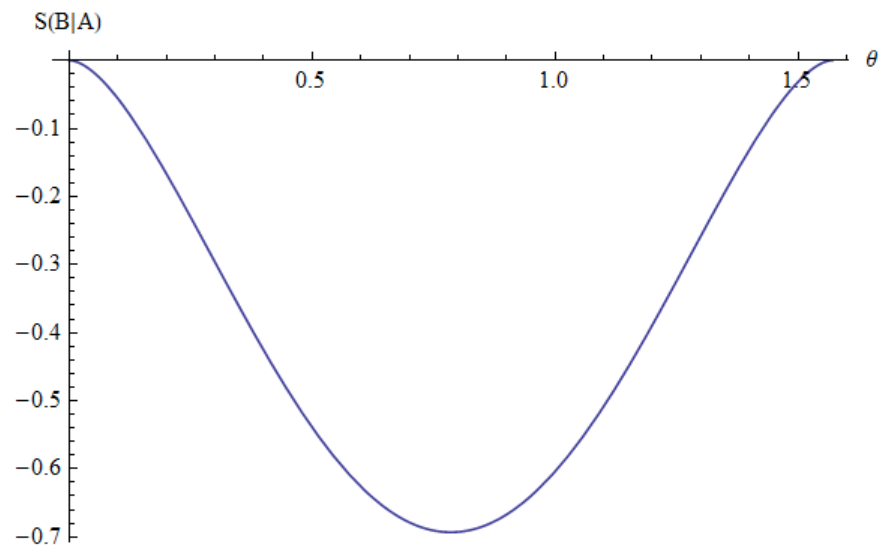
\includegraphics{figures/cond_ent_plot.png}
\end{center}

Actually the plot demonstrates lots of aspects of the conditional entropy. For example, we can easily see that the minimum is close to $-ln2$. This is not an accident since is common among the so called maximally entangled states. In particular, $\theta= \pi /2$ will give this type of state.